\subsection{Cross Sections as a function of the proton angle}
%Results in $\theta_{p}$ 

Figure~\ref{figure:xsec_proton_theta} shows the observed differential cross section as a function of $\theta_{p}$ for interactions on each of the nuclear targets, respectively.
$\theta_{p}$ is the opening angle of the proton direction relative to the beam direction.  The uncertainties broken down by source for both the absolute cross sections and the cross section ratios as a function of $\theta_p$ can be found in Fig.~\ref{fig:xsec_err_proton_theta}.

\begin{figure}[h]  
	\centering
   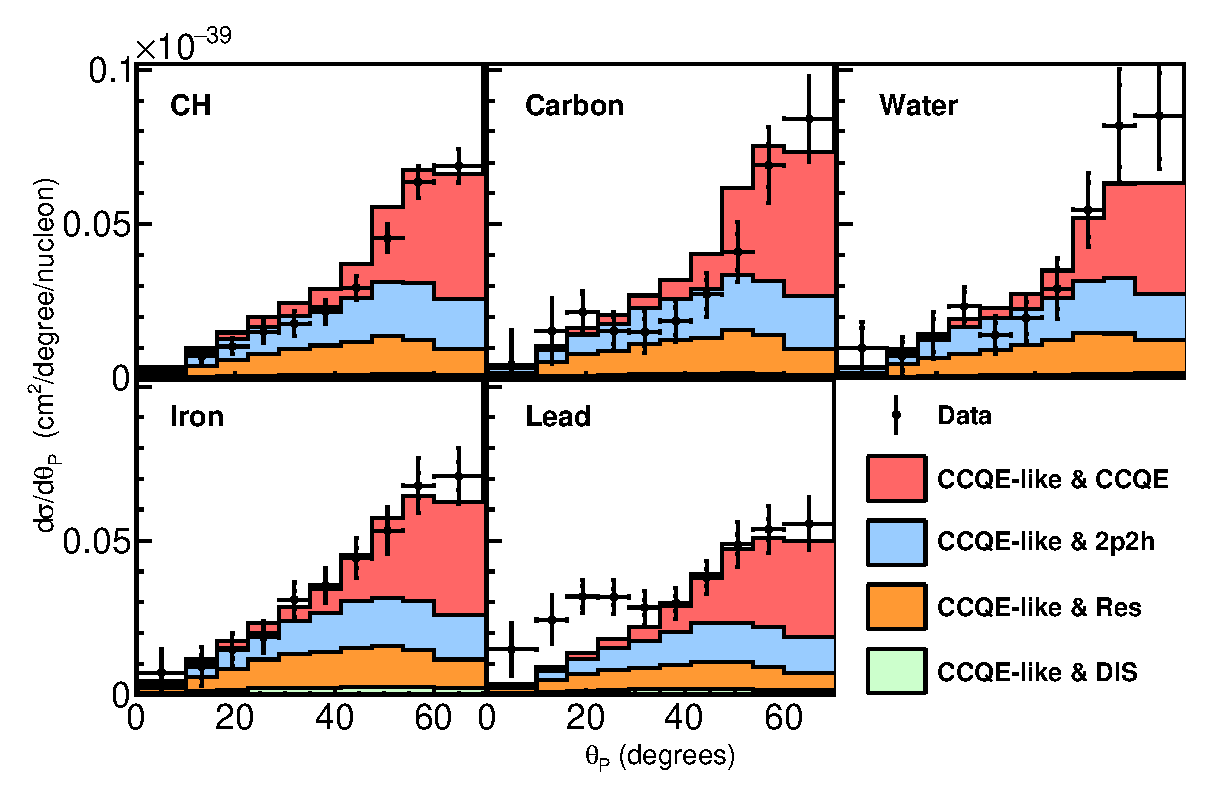
\includegraphics[width=\linewidth]{Figures/xsec_five_square/proton_theta.eps}
	\caption{The differential cross section as a function of $\theta_p$ for CH, C, H$_{2}$O, Fe, and Pb targets, along with the predictions for the different quasielastic-like signal processes.}
	\label{figure:xsec_proton_theta}
\end{figure}

The data is fairly well modeled by the MINERvA tune for each target except Pb.  Note the inflection around 40 degrees where the CCQE process tends to kick in.  For the data taken on Pb, relative to the other targets, it seems that a different process is significant below 40 degrees that is not well modeled by the MINERvA tune.  

%The data taken on the Pb target shows a significant enhancement at angles below 40 degrees relative to MnvGENIE.  The data have a different shape than what is seen in the other targets, exhibiting a possible two-component behavior.  This indicates something new is happening as the nuclear size grows past what is seen in Fe.

A range of models are compared to the data in terms of the differential cross section as a function of $\theta_{p}$ for each of the nuclear targets in Fig.~\ref{fig:models_proton_theta}.
  NEUT tends to have significantly more cross section in the intermediate $\theta_{p}$ region dominated by 2p2h resonant events.  For the larger targets, NEUT and the hN versions of GENIE exhibit significantly higher cross sections than the data at all but the smallest angle. Besides NuWro SF, the other models tend to be closer to the data relative to the MINERvA tune in the small angle region making it seem less like a process is missing in the models.  The \chisq\ between the cross sections and the models can be found in Table~\ref{tab:protontheta}.

% comparisons to generators proton_theta

\begin{figure}
    \centering
 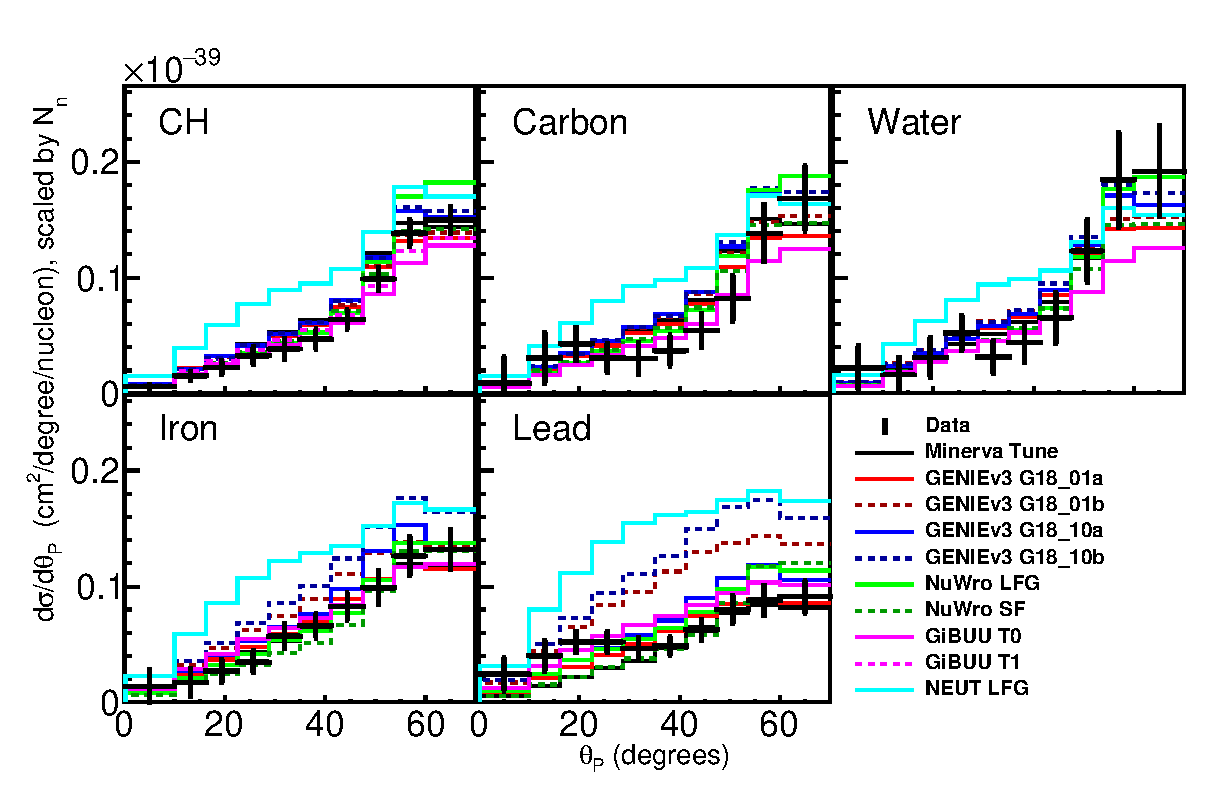
\includegraphics[width=\linewidth]{Figures/gencompare/proton_theta_5square.eps}
    \caption{Cross section measurements and predictions as a function of $\theta_p$ for different targets and for a selection of different generator and model choices.}
    \label{fig:models_proton_theta}
\end{figure}

The ratio of the differential cross section as a function of  $\theta_{p}$ for each nuclear target (C, H$_{2}$O, Fe, Pb) to that for scintillator is shown in 
Fig.~\ref{Figure:Gencompare_proton_theta_ratio}. For the ratios as a function of $\theta_{p}$, there is qualitative agreement between the data and the MINERvA tune except for the distributions for the Pb target.  For Pb, NEUT, GiBUU, and the hN versions of GENIE agree with the data ratio at low angle but exhibit larger ratios than the data at large angles.  NuWro and the hA versions of GENIE agree well with the data ratio at larger angles and tend to underpredict the data at lower angles.
The \chisq\ between the cross section ratios and the models can be found in Table~\ref{tab:protontheta}.

\begin{figure}
    \centering
 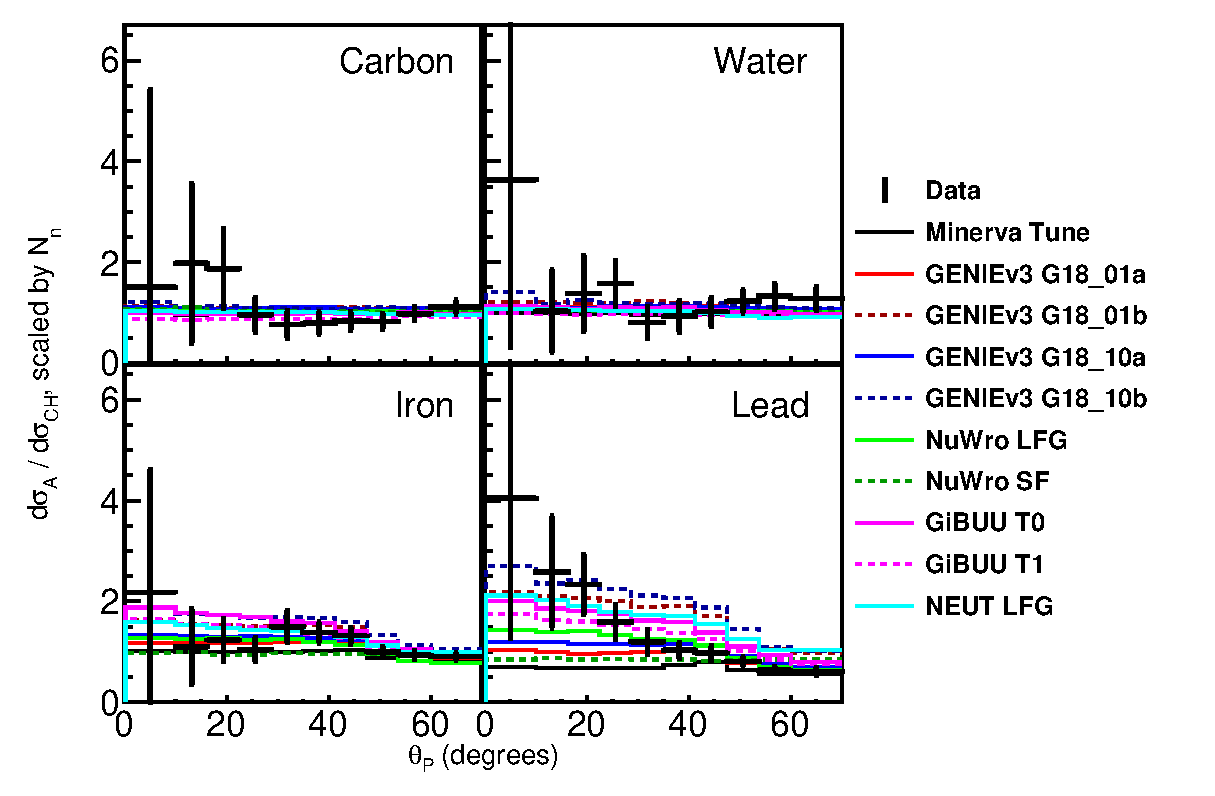
\includegraphics[width=\linewidth]{Figures/gencompare/proton_theta_4square.eps}
    \caption{Cross-section ratio as a function of proton angle, for several generators and multiple targets.  Changes to the FSI model (GENIE ``a'' to ``b'') in GENIE change the cross section ratio most at low proton angles, and those changes are larger than changes to the 2p2h model (GiBUU T0 to GiBUU T1) or changes to the initial state (GENIE 1 to GENIE 10) or (NuWro LFG to NuWro SF).}
\label{Figure:Gencompare_proton_theta_ratio}
\end{figure}
